% Matteo Kumar - Leonard Schatt
% Physikalisches Praktikum

% Anhang A

\chapter{Anhang}
\label{chap:anhangA}
\section{Nanoröhrchen}
\begin{figure}
    \centering
    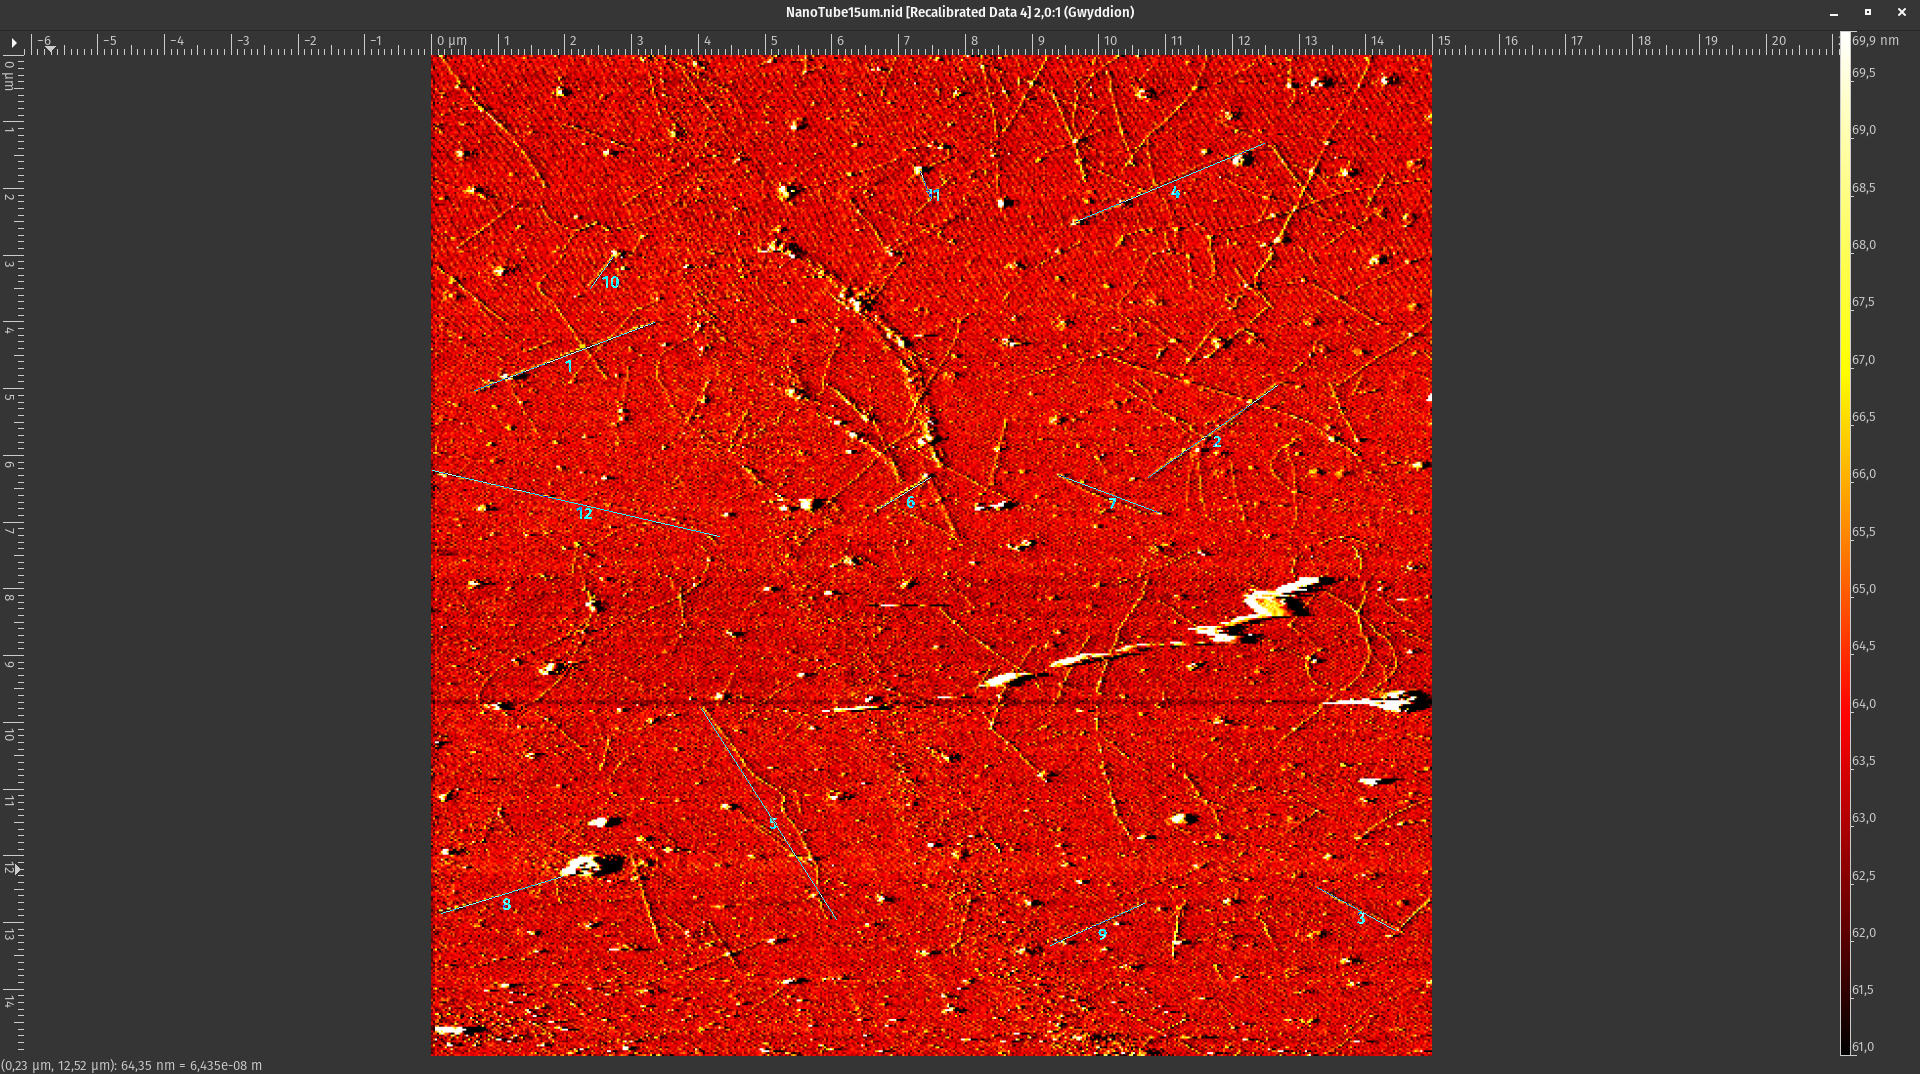
\includegraphics[width = \linewidth]{Bilder/Nanotubes/NanoTube15umLaenge2.png}
    \caption{Nanoröhrchen und die zur Vermessung der Länge gewählten Distanzen}
    \label{Nanotube20Mess}
\end{figure}

\begin{figure}
    \centering
    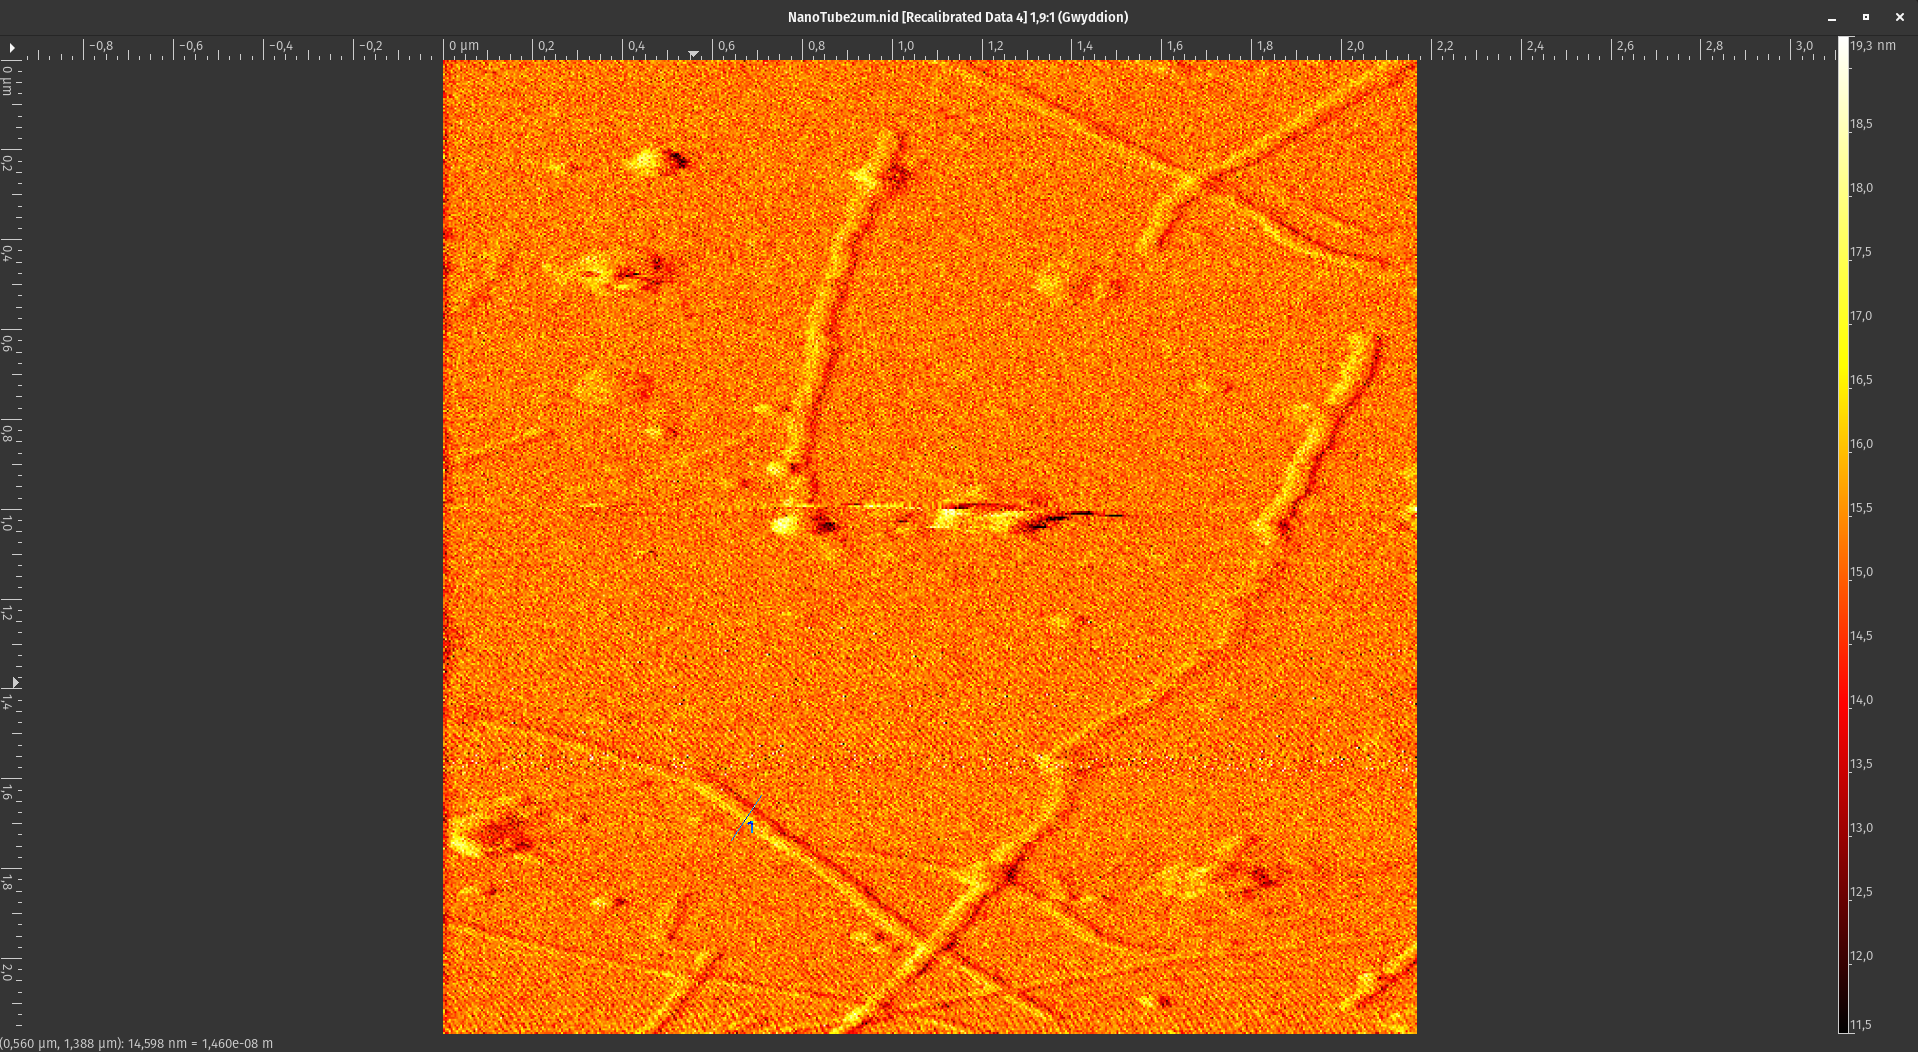
\includegraphics[width = \linewidth]{Bilder/Nanotubes/NanotubesBreiteHoehe2.png}
    \caption{Nanoröhrchen und die zur Vermessung des Radius gewählten Distanzen}
    \label{NanoRadius}
\end{figure}
